\chapter{Integration theory}

\section{Orientations of vector spaces}

Let \(V\) be a real vector space of dimension \(n\geq 0\). Then:
\begin{itemize}
    \item \(\Lambda^n V^\star\) is a 1 dimensional vector space 
    \item \(\Lambda^nV^\star\setminus\{0\}\), carries an action of  \(\R_+\coloneqq [0,\infty)\)
          by scaling \((\lambda,\omega)\mapsto \lambda \omega\). The quotient \(\Lambda^n V^\star\setminus\{0\}/\R_+\) is a 
          is a set with two elements, with discrete topology. 
    \item Let \(B=\{v_1,\dots,v_n\},\tilde{B}=\{\tilde{v_1},\dots,\tilde{v_n}\}\). We write \(M_B^{\tilde{B}}\) for the transition matrix 
          i.e. \[v_i=\sum_{j=1}^n (M_B^{\tilde{B}})_ij \tilde{v}_j\]
\end{itemize}

\dhighlight{Exercise:} If \(B^\star,\tilde{B}^\star\) are the dual basis, then \(M_{B^\star}^{\tilde{B}^\star}=(M_B^{\tilde{B}})^\star\).

\begin{definition*}\marginnote{Only for this lecture}
    Given \(V\) as above, we write \(B\sim \tilde{B}\iff \det(M_B^{\tilde{B}})>0\).
\end{definition*}

Clearly this is an equivalence relation.

\begin{lemma}\label{lem:11.1}
    Let \(V\) be a finite dimensional vector space. TFAE:
    \begin{enumerate}
        \item[(i)] an equivalence class \([B]\) of bases for \(V\)
        \item[(ii)] an equivalence class \([B^\star]\) of bases for \(V^\star\)
        \item[(iii)] an element of \(\Lambda^{\text{top}}V^\star\setminus \{0\}\) \marginnote{\(\Lambda^{\text{top}}V\setminus \{0\}=\Lambda^{n}V\setminus \{0\}\), where \(n=\dim V\). He also didn't use a star after \(V\)}.  
    \end{enumerate}
    We call any one of these equivalent pieces of data an \dhighlight{orientation}.
\end{lemma}

\begin{proof}
    \((i)\iff(ii)\) is clear.

    (ii) \(\implies\) (iii). If \(B=\{v_1,\dots,v_n\}\) basis of \(V^\star\), then 
    \(v_1\wedge \dots\wedge v_n\in \Lambda^{\text{top}}V^\star\setminus\{0\}\). If \(\tilde{B}=\{\tilde{v}_1,\dots,\tilde{v}_n\}\)
    is any other basis, then \(\tilde{v}_1\wedge \dots\wedge \tilde{v}_n=\det(M_{B}^{\tilde{B}})v_1\wedge \dots\wedge v_n\).
\end{proof}

\begin{definition*}[Interior multiplication]
    Let \(V\) be a finite-dimensional, \(R\)-vector space. Fix \(v\in V,\omega\in \Lambda^k V^\star\). Then we 
    let \(\iota_v\omega(\cdot,\dots\cdot)\coloneqq \omega(v,\cdot,\dots,\cdot)\in \Lambda^{k-1}V^\star\)
\end{definition*}

\begin{lemma}[Induced orientation]\label{lem:11.2}
    Let \(V\) be a finite-dimensional, \(\R\)-vector space. Let \(j:H\hookrightarrow V\) be a \(n-1\) dimensional 
    subspace. Fix an orientation \(\omega\in \Lambda^{n}V^\star\setminus\{0\}\). Fix \(v\in V\) transverse to \(H\).
    \begin{figure}[H]\label{fig:11.1}
        \centering
        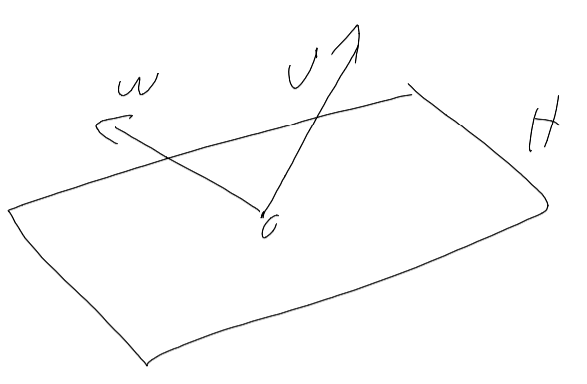
\includegraphics[width=.7\textwidth]{sketch_11_01.png}
        \caption{Sketch 11.1}
    \end{figure}  
    Then:
    \begin{enumerate}
        \item[(i)] \(\iota_v\omega\restrict{H}=j^\star(\iota_v\omega)\in \Lambda^{n-1}H^\star\) is an orientation on \(H\)\marginnote{it is non-zero!}
        \item[(ii)] the orientation from (i) only depends on the connected component of \(V\setminus H\) in which \(v\) is contained. 
    \end{enumerate} 
\end{lemma}

\begin{proof}
    \dhighlight{(i)} need to check, that \(j^\star(\iota_v\omega)\neq 0\).  Pick a basis \(\{y_1,\dots,y_{n-1}\}\) for \(H\). Then 
    \begin{align*}
        (j^\star(\iota_v\omega))(y_1,\dots,y_{n-1})=\omega(v,y_1,\dots,y_{n-1})\neq 0
    \end{align*}
    since \(v,y_1,\dots,y_{n-1}\) is a basis for \(V\).
    
    \dhighlight{(ii)} If \(v,w\) are in the same connected component, then \(v=\lambda w\sum_{i=1}^n a_iy_i\), where 
    \(\lambda>0,a_1,\dots,a_{n-1}\). Then 
    \begin{align*}
        \iota_v\omega(y_1,\dots,y_n)&=\omega(v,y_1,\dots,y_{n-1})\\
        &=\omega(\lambda w+ \sum_{i=1}^{n-1}a_i y_i,y_1,\dots,y_{n-1})\\
        &=\omega(\lambda w,y_1,\dots,y_{n-1})+\underbrace{\omega(\sum_{i=1}^{n-1}a_iy_i,y_1,\dots,y_{n-1})}_{=0}\\
        &=\lambda\omega(w,y_1,\dots,y_{n-1})\\
        &=\lambda\iota_w(y_1,\dots,y_{n-1})\\
        \implies \iota_v\omega&=\lambda\iota_w\omega
    \end{align*}
\end{proof}

\section{Orientations of smooth manifolds}

\begin{definition*}
    Let \(M\) be a smooth manifold.  An \dhighlight{orientation} is a smooth section 
    \(\sigma\in\Gamma^1(\Lambda^{\text{top}}T^\star M)=\Omega^{\text{top}}(M)\), which is non-vanishing, modulo the 
    equivalence relation \(\sigma\sim\sigma'\iff \exists f:M\to\R_+,\sigma'=f\sigma\).
    
    We call the data of a manifold + an orientation an \dhighlight{oriented manifold}.
\end{definition*}

\begin{remark}[for topology enthusiast]\marginnote{non examable, proved by approximation}
    The following definitions are equivalent to the one above:
    \begin{enumerate}
        \item[(i)] a continuous \(\sigma\) of \(\Lambda^{\text{top}}T^\star M\), 
                   which is non-vanishing, modulo \(\sigma\sim\sigma'\iff \exists f:M\to\R_+\), continuous, \(\sigma'=f\sigma\). 
        \item[(ii)] A section of the fiber bundle \((\Lambda^{\text{top}}T^\star M\setminus 0_M)/\R_+\stackrel{\pi}{\to}M\ni p\)
                    \(\pi^{-1}(p)=(\Lambda^{\text{top}}T_p^\star M\setminus 0_M)/\R_+\)            
    \end{enumerate}
\end{remark}

\begin{example}
    \(\R^n,\omega_0\coloneqq dx_1\wedge\dots\wedge dx_n\in\Omega^n(\R^n)\). We call 
    \(\omega_0\) the \dhighlight{canonical} orientation.
\end{example}

\begin{example}[Non-example / Warning]
    Not all manifolds admit an orientation! E.g. \(\R\bP^{2n}\) are non-orientable, similarly the Möbius band.
\end{example}

If we have a manifold, the \(TM\) is also a manifold and it is always orientable!

\begin{lemma}\label{lem:11.3}
    Let \(M\) be a manifold and let \(j:H\hookrightarrow M\) be a codimension \(1\) submanifold. Fix an orientation 
    \(\omega\) on \(M\). Let \(V\) be a vector field along \(H\), which is transverse to \(H\), i.e. a section \(V\) 
    \((\underbrace{j^\star TM}_{\equiv TM\restrict{H}}\to H)\) s.t. \(\sigma_p\perp T_p H, T_pH\subset T_p M\).
    Then 
    \begin{enumerate}
        \item[(i)] \(j^\star\iota_V\omega \in \Omega^{\text{top}}\) is an orientation
        \item[(ii)] if \(W\) is a vector field along \(H\), transverse to \(H\), such that \(V_p,W_p\) lie in the same connected component
                    of \(T_pM\setminus T_pH\) for all \(p\in H\). Then \(j^\star(\iota_V\omega)=j^\star(\iota_W\omega)\).   
    \end{enumerate}
    We call this orientation the \dhighlight{induced orientation} (depends on \(H\subset M,\omega,V\)).
\end{lemma}

\begin{proof}
    Immediate corollary of lemma \ref{lem:11.2}.
\end{proof}

\begin{definition*}
    Let \(M\) be a manifold with boundary. A vector \(v\in T_pM,p\in\partial M\subset M\) is said to be 
    \dhighlight{inward-pointing} if there exists a curve \(\gamma:[0,\epsilon)\to M,\dot{\gamma}(0)=v\notin T_p \partial M\). We say 
    \(w\in T_pM\) is \dhighlight{outward pointing} if \(-w\) is inward-pointing. 
\end{definition*}

\dhighlight{Observe:} Any positive linear combination of inward-pointing vectors is inward-pointing.
If we have \(a_1,\dots,a_n\geq 0,\sum a_i=1\), \(v_1,\dots,v_n\) inward-pointing at \(p\), then so is \(\sum_{a_i}v_i\).


\begin{lemma}\label{lem:11.4}
    Let \(M\) be a manifold with non-empty boundary.
    \begin{enumerate}
        \item[(i)] There exists an inward pointing vector field (also outward-pointing vector fields)
        \item[(ii)] If \(\omega\in\Lambda^{\text{top}}(M)\) orientation on \(M\), \(Z\) any outward-pointing vector field, then 
                    \(j^\star(\iota_Z\omega)\in \Omega^{\text{top}}\), \(j:\partial M\hookrightarrow M\), is an orientation. 
    \end{enumerate}
    We call \(j^\star(\iota_Z\omega)\in\Omega^{\text{top}}(\partial M)\) the \dhighlight{induced / Stokes orientation} on \(\partial M\). It does not depend on the choice of outward pointing vector field.
\end{lemma}


\begin{proof}
    \dhighlight{(ii):} Immediate consequence of lemma \ref{lem:11.3}.

    \dhighlight{(i):} We seek \(Z\) a section of \((\underbrace{j^\star TM}_{=\partial M\substack{\times\\M} TM}\to \partial M)\)
    s.t. \(\forall p\in \partial M, Z_p\in T_p\partial M\subset T_p M\), \(Z_p\) lies in the \highlight{canonical} component of 
    \(T_p M \setminus T_p \partial M\). Choose a covering of \(\partial M\) by charts \((U_\alpha,\varphi_\alpha),\varphi_\alpha:U_\alpha\to\bH^n\).
    Choose a subordinate partition of unity \(\{\eta_\alpha\}_{\alpha}\).

    Let \(Z_0\in\Gamma(\bH^n),Z_0=\partial_{x_n}\)
    \begin{figure}[H]\label{fig:11.2}
        \centering
        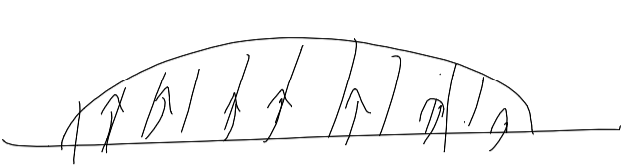
\includegraphics[width=.7\textwidth]{sketch_11_02.png}
        \caption{Sketch 11.2}
    \end{figure}
    Let \(Z=\sum_{\alpha}\eta_\alpha(d\varphi_{\alpha}^{-1}(Z_0))\) this works 
    because of the previous observation about positive combinations of inward pointing vectors.    
\end{proof}

\begin{example}
    Let \(B^{n+1}(1)\subset \R^{n+1},\partial B^{n+1}(1)=S^n\).
    We have \(Z=x_1\partial_{x_1}+\dots+x_n\partial_{x_n}\). Clearly \(\forall p\in S^n, Z_p\perp T_p S^n\)
    \begin{figure}[H]\label{fig:11.3}
        \centering
        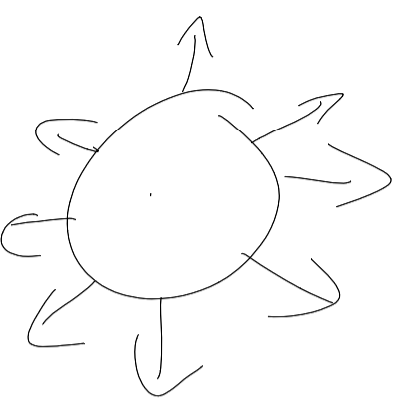
\includegraphics[width=.7\textwidth]{sketch_11_03.png}
        \caption{Sketch 11.3}
    \end{figure}
    \(\implies\) By lemma \ref{lem:11.4}, \(i_z \omega_0\) on \(S^n\).
\end{example}

\markeol{25}

\beginlecture{26}{21.01.2025}
\dhighlight{Exam announcement:}
\begin{itemize}
    \item 1 Problem is drawn from homework (maybe slightly simplified)
    \item both exams are indented to be of similar difficulty
    \item Everything up to this week is relevant
    \item Prepare for the exam by doing old exams questions 
    \item The exam consists of problems, not just repeating proves of the class, however the proof ideas might be useful!
    \item 2 hours
    \item Please look at the course webpage! 
\end{itemize}

\begin{definition*}
    Let \(M\) be an oriented manifold. We say that a chart \((U,\varphi)\) is positively/ negatively 
    oriented if, w.r.t to local coordinates \(x_1,\dots,x_n\), \(\varphi^\star(dx_1,\dots,dx_n)\in\Omega^{\text{top}}(\Omega)(U)\) agrees / disagrees with 
    the orientation of \(M\) (restricted to \(U\)). 
\end{definition*}

In this setting, any chart is either positively or negatively oriented! Let \(r:\R^n\to\R^n,(x_1,\dots,x_n)\mapsto (-x_1,\dots,x_n)\).
Then observe that \((U,\varphi)\) \(\pm\) oriented  iff \((U,r\circ \varphi)\) is \(\mp\) oriented.

Recall a Riemannian manifold \((M,g)\) is a manifold \(M\) + a section \(g\)
\(\Gamma(T^{\otimes 2}T^\star M)\) such that
\((T_p M,g_p)\) is an inner product space.  

\dhighlight{Exercise: }\marginnote{he would like us to do this exercise, it is insightful and important, but belongs to section9}
Let \((M,g)\) be a Riemannian manifold. Given \(p\in M\), there exists a local orthonormal 
frame at \(p\) (i.e. \(U\ni p,e_1,\dots e_n\in \Gamma(TM\restrict{U}),g_q(e_i,e_j)=\delta_{ij}\forall q\in U\)).
\begin{proof}[proof idea]\marginnote{Might very well be important for the exam}
    Apply the Gram-Schmitt process, all the operations are smooth. Take a local frame through this process and show it works.
\end{proof}

For reasons which will become apparent later today, a nowhere-zero top-form \(\omega\in\Omega^{\text{top}}(M)\)
defines an orientation and is often called a \dhighlight{volume form}.

\begin{lemma}\label{lem:11.5}
    Let \((M,g)\) be a orientable Riemannian manifold. Then there exists a unique top form 
    \(\omega_g\in\Omega^{\text{top}}(M)\), with the property that \((\omega_g)_p(e_1,\dots,e_n)\), where \(\{e_1,\dots,e_n\}=1\) is an orthonormal basis at \(p\).
\end{lemma}

\begin{proof}[Proof sketch]
    Fix \(p\in M\). Let \((\epsilon^1,\dots,\epsilon^n)\) be a local, orthonormal, co-frame. Define 
    \(\omega_g\coloneqq \epsilon^1\wedge\dots\wedge \epsilon^n\) near \(p\). Suppose that 
    \(\tilde{\epsilon}^1,\dots,\tilde{\epsilon}^n\) is another orthonormal co-frame. Let \(M_{B}^{\tilde{B}}\)
    be the transition matrix. We have \(\epsilon^{1}\wedge \dots\wedge \epsilon^n=\det(M_{B}^{\tilde{B}})\tilde{\epsilon}^1\wedge\dots\wedge\tilde{\epsilon}^n\). Since 
    \(\{\epsilon\},\{\tilde{\epsilon}\},M_B^{\tilde{B}}\in O(TM,g)\), i.e. \(M_B^{\tilde{B}}(q)\in (T_q M, g_q)\).
    Therefore \(\det(M_{B}^{\tilde{B}})=\pm1\). Choosing the correct orientation concludes the proof.
\end{proof}

\section{Integration on manifolds}

In Analysis 1-3, you developed the notion of the integral of function \(f:\R^n\to \R\).

\[\int_{\R^n} fdx_1,\dots,fx_m\]
\(\supp(f)\) compact, \(f\) measurable.

\dhighlight{Careful, this is not invariant under diffeomorphism!} This notion makes no sense in our category.

\begin{example}
    \begin{figure}[H]\label{fig:11.4}
        \centering
        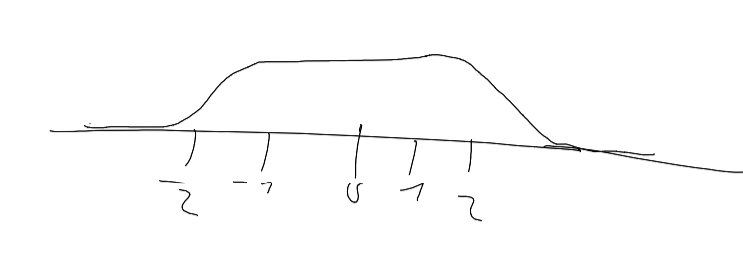
\includegraphics[width=.7\textwidth]{sketch_11_04.png}
        \caption{Sketch 11.4}
    \end{figure}
    \(\int fdx\approx 2\). Consider \(\phi:\R\to\R,x\mapsto x/100\)
    \[\int_\R \phi^\star f=\int_\R (f\circ \phi)\approx 200.\]
\end{example}
\dhighlight{Solution:} Instead of integrating functions, we should be integrating top forms.

\dhighlight{Key lemma}: 10.10 (d) Recall

\(\phi M\to N,\varphi^\star(fdy_1\wedge\dots\wedge dy_n)(d\phi)dx_1,\dots,dx_n\).
The change of variable is backed in the pullback of top forms.

\begin{definition*}
    Let \(U\subset\R^n/\bH^n\). Let \(\sigma=f(x_1,\dots,x_n)dx_1,\wedge\dots\wedge x_n\in\Omega^{\text{top}}(U)\)
    be a \highlight{compactly supported} top form. We define:
    \[ \int_U sigma\coloneqq \int_U f(x_1,\dots,x_n)dx_1,\dots,dx_n,\]
    where the right side is the usual integral from analysis 2/3.
\end{definition*}

\begin{lemma}\label{lem:11.6}
    Let \(U,V\subset \R^n/\bH^n\). Let \(\varphi:U\to V\) be a diffeomorphism. Given \(\eta\) compactly supported,
    we have \[\int_U \varphi^\star \eta=\begin{cases}
        \int_V \eta & \text{if } \sigma\text{ orientated positively}\\
        -\int_V \eta & \text{if } \sigma\text{ orientated negatively}
    \end{cases}\] 
\end{lemma}
\begin{proof}
    \begin{align*}
        \int_U \varphi^\star \eta&=\int_U \varphi^\star(fd_y1\wedge \dots\wedge dy_n)\\
        &\stackrel{\text{Lemma \ref{lem:1.10} (d)}}{=}\int_U (f\circ \varphi)(\det d\varphi) dx_1\wedge \dots dx_n\\
        &= \int_U (f\circ \varphi)(\det d\varphi) dx_1\dots dx_n\\
        &=(\pm)\int_U (f\circ \varphi)|\det d\varphi| dx_1\dots dx_n\\
        &=(\pm) \int_V f dy_1,\dots,dy_n
    \end{align*}
    by the change of variable theorem and 
    \begin{align*}
        (\pm) \int_V f dy_1,\dots,dy_n &= \int_V f dy_1\wedge\dots\wedge dy_n\\
        &=\int_V \eta\qedhere
    \end{align*}
\end{proof}


\begin{lemma}[Provisional definition, only for this lecture]\label{lem:11.7}
    Let \(M\) be a smooth manifold, possibly with boundary Let \(\omega\in \Omega^{\text{top}}(M)\). Suppose that:
    \begin{enumerate}
        \item[(i)] \(\supp(\omega)\) is compact 
        \item[(ii)] there exists a chart \((U,\varphi)\) such that \(\supp(\omega)\subset U\).  
    \end{enumerate}
    Then \(\int_M\omega\coloneqq \pm \int_{\varphi(U)}(\varphi^{-1})^\star \omega\)
    where we choose \(\pm\) depending on wether \((U,\varphi)\) is positively or negative oriented.
    This expression does not depend on the choice of chart \((U,\varphi)\).
\end{lemma}
\begin{proof}
    Let \((V,\psi)\) be another such chart. For simplicity, assume that 
    both are positively oriented. Then we have: 
    \begin{align*}
        \int_{\psi(V)}(\psi^{-1})^\star \omega&=\int_{\psi(V\cap V)}(\psi^{-1})^\star \omega\\
        &=\int_{\varphi(U\cap V)} (\psi\circ\phi^{-1})^\star (\psi^{-1})^\star\omega\\
        &=\int_{\varphi(U\cap V)}(\varphi^{-1})^\star \psi^\star(\psi^{-1})^\star \omega\\
        &=\int_{\varphi(U)}(\varphi^{-1})^\star \omega \qedhere
    \end{align*}
\end{proof}

\begin{lemma}\label{lem:11.8}
    Let \(M\) be an orientated, smooth \(n\) manifold, possibly with boundary. Let 
    \(\omega\in \Omega^n(M)\). Suppose that: 
    \begin{enumerate}
        \item[(i)] \(\supp\omega\) is compact
        \item[(ii)] \(\{U_i,\varphi_i\}_{i=1}^N\) such that \(\supp\omega\subset \bigcup_{i=1}^N U_i\) \marginnote{Unproblematic, since \(\supp \omega\) is compact} 
        \item[(iii)] \(\{\eta_i\}_{i=1}^N\) be a partition of unity subordinate to \(\{U_i\}_{i=1}^N\). 
    \end{enumerate}
    We define 
    \[\int_M \omega\coloneqq \sum_{i=1}^N \int_{M}\eta_i\omega=\sum_{i=1}^N \int_{\varphi_i(U_i)}(\varphi^{-1})^\star\eta_i\omega\]
    This definition does not depend on the choice of \(\{(U_i,\varphi_i)\}_i,\{\eta_i\}\)\marginnote{Please remember this for for the exam}
\end{lemma}
\begin{proof}
    Let \(\{(\tilde{U}_j,\tilde{\varphi}_j)\}_{j=1}^{\tilde{N}},\{\tilde{\eta}_j\}_{j=1}^{\tilde{N}}\) be another such choice.
    Then observe that 
    \begin{align*}
        \int_M \eta_i \omega &= \int_M \left(\sum_{j=1}^{\tilde{N}\tilde{\eta}_i}\right)\eta_i\omega\\
        &=\sum_{j=1}^{\tilde{N}}\int_{M}(\tilde{\eta}_j\eta_i)\omega.
    \end{align*}
    Similarly \[\int_m \tilde{\eta}_j\omega=\sum_{i=1}^N\int_M(\tilde(\eta)_j\eta_i)\omega.\]
    Now 
    \begin{align*}
        \int_M\omega&=\sum_{i=1}^N\int_M \eta_i \omega =\sum_{i=1}^N\sum_{j=1}^{\tilde{N}}\int_M(\tilde{\eta}_j\eta_i)\omega\\
        &=\sum_{j=1}^{\tilde{N}}\sum_{i=1}^N\int_M(\tilde{\eta}_j\eta_i)\omega=\sum_{j=1}^{\tilde{N}}\int_M \tilde{\eta}_j \omega \eqqcolon \int_M \omega \qedhere
    \end{align*}
\end{proof}

\begin{remark}
    \begin{itemize}
        \item All of the familiar properties of the integral in \(\R^n\) remain true, but are left as an exercise. E.g.
                \[\int_M a\omega +b\eta=\int_M a\omega +\int_M b\eta\]
        \item You can do measure theory on manifold, but this is not what we have done today. Integration of smooth functions in \(\R^n\) can be generalized in two ways \begin{itemize}
            \item integration on manifolds 
            \item integrations of measurable functions in \(\R^n\)
        \end{itemize}
    \end{itemize}
\end{remark}

\markeol{26}
\beginlecture{27}{24.01.2025}

Klausureinsicht\footnote{Revision / discussion of the exam grades} for exam number one: SR0.011 at 12:30-13:30 on thursday 13.02.25.
Last lecture he said it exam will be problem based, but he might ask us to prove a step of some proof of the lecture.

\begin{remark}[Integration on zero-dimensional manifolds]\marginnote{This is important (in practice)}
    \begin{itemize}
        \item By convention, if \(V\) is a 0-dim. vector space, an orientation \(o_V\) on \(V\) is an element \(o_V\in \{\pm 1\}\)
        \item Hence if \(M\) is a 0-dim manifold, an orientation is the assignment of \(\pm 1\) to each element of \(M\) (\(\sigma\in \Omega^0(M)=C^\infty(M)\), nowhere zero)
        \item If \(M\) is a zero-dimensional oriented manifold, \(\eta\in \Omega^0(M)=C^\infty(M)\), compactly supported. Then \[\int_M \eta=\sum_{p\in M}(\pm)\eta(p)\] where \(\pm\) depends on wether \(p\) is oriented \(\pm\).  
    \end{itemize}
\end{remark}

\section{Stokes' theorem}

\begin{theorem}[Stokes's theorem]\label{thm:11.9}
    Let \(M\) be an oriented \(n\)-manifold with boundary. Let 
    \(\omega\in \Omega^{n-1}(M)\) be a compactly supported \(n-1\) form. Then 
    \[\int_M \underbrace{d\omega}_{\in \Omega^n(M)}=\int_{\partial M} \omega.\]
\end{theorem}

\begin{remark}
    \begin{itemize}
        \item \(\partial M =\emptyset\) is allowed 
        \item it is understood that \(\partial M\) carries the induced boundary orientation from section 11.1 (outward pointing, stokes orientation)
        \item the expression \(\int_{\partial M}\omega\) secretly means \[\int_{\partial M} j^\star \omega,j:\partial M \hookrightarrow M\]
    \end{itemize}
\end{remark}

\begin{lemma}\label{lem:11.10}
    Endow \(\partial \bH^n\) with the induced orientation. The map \(\R^{n-1}\to\partial \bH^n\),
    which sends \[(x_1,\dots,x_n)\mapsto (x_1,\dots,x_n,0)\]
    is orientation preserving if \(n\) is even and orientation reversing if \(n\) is odd.
\end{lemma}

\begin{proof}
    By definition, orientation on \(\partial \bH^n\) \(i_{-\partial_{x_n}}w_0=i_{(-\partial_{x_n})}dx_1\wedge\dots\wedge dx_n = (-1)^{n}i_{\partial_{x_n}}dx_1\wedge \dots \wedge dx_{n-1}\).
    \[j^\star((-1)^ndx_1\wedge \dots \wedge dx_{n-1})=(-1)^n dx_1\wedge\dots \wedge dx_{n-1}\qedhere\]
\end{proof}
Proof of Stokes theorem, see \cite{smooth_manifolds} theorem 16.11.

\begin{proof}[Proof when \(M=\bH^n\)]
Since \(\omega\) is compactly supported, \(\supp \omega\subset \underbrace{[-R,R]\times\dots\times  [-R,R]}_{n-1\text{ times}}\times [0,R]\) 
\begin{figure}[H]\label{fig:11.5}
    \centering
    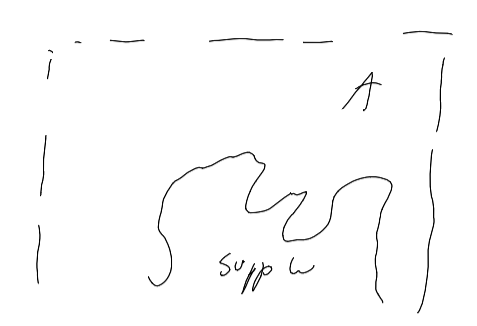
\includegraphics[width=.7\textwidth]{sketch_11_05.png}
    \caption{Sketch 11.5}
\end{figure}   
We can write \(\omega=\sum_{i=1}^n\omega_i dx_i\wedge \dots \wedge \hat{dx_i}\wedge \dots \wedge dx_n\).\marginnote{\(\hat{dx_i}\) means we are omitting this term}
We can now compute 
\begin{align*}
    d\omega&=\sum_{i=1}^n\sum_{j=1}^n \partial_{x_j} w_i dx_j\wedge dx_1\dots\wedge dx_i\dots \wedge dx_n\\
    &=\sum_{i=1}^n(-1)^{i-1}\partial_{x_i}w_i dx_1\wedge \dots\wedge dx_n
\end{align*}
By definition 
\begin{align*}
    \int_{\bH^n} d\omega &=\int_{A} d\omega=\int_A \sum_{i=1}^n(-1)^{i-1}\partial_{x_i}w_i dx_1\wedge \dots\wedge dx_n\\
    &= \sum_{i=1}^{n} (-1)^{i-1}\int_A \partial_{x_i}w_i dx_1\dots dx_n=\sum_{i=1}^n (-1)^{i-1}\int_0^R\int_{-R}^R\dots \int_{-R}^R\partial_{x_i}w_i dx_1\dots dx_n =(\star)
\end{align*}
\dhighlight{Observe:} \[\int_\R^R \partial_{x_i}\omega_i dx_i=\omega_i\mid_{-R}^R=0\] 
\begin{align*}
    (\star) &= (-1)^{n-1} \int_0^R\dots\int_{-R}^R \partial_{x_n}\omega_n dx_1\dots dx_n\\
    &=(-1)^n\int_{-R}^R\dots \int_{-R}^R \omega_n(x_1,\dots,x_{n-1},0) dx_1\dots dx_n
\end{align*}

Meanwhile 
\begin{align*}
    \int_{\partial \bH^n}\omega&=\int_{\partial \bH^n\cap A}\sum_{i=1}^n\omega_i dx_1\wedge \dots\wedge \hat{dx_i}\wedge \dots \wedge dx_n
\end{align*}
Note that, since \(x_n\equiv 0\partial\) on \(\bH^n\), \(dx_n\equiv 0\) on \(\partial \bH^n\)
\begin{align*}
    \implies \int_{\partial \bH^n}\omega=\int_{A\cap \partial \bH^n}\omega_n dx_1\wedge \dots\wedge  dx_{n-1} 
\end{align*}
But now, by lemma \ref{lem:11.10}, we have 
\begin{align*}
    \int_{A\cap \partial \bH^n} \omega_n dx_1\wedge \dots \wedge dx_{n-1}&=(-1)^n \int_{[-R,R]^{n-1}}\omega_ndx_1\wedge \dots \wedge dx_{n-1}\\
    &= (-1)^n \int_{-R}^R\dots \int_{-R}^R \omega_n (x_1,\dots,x_{n-1},0)dx_1\dots dx_{n-1}
\end{align*} 
\end{proof}

\begin{proof}[Proof when \(M=\R^n\)]
    As before \(\omega=\sum_{i=1}^n\omega_i dx_1\wedge \dots \wedge \hat{dx_i}\wedge \dots\wedge dx_n\),
    \(d\omega=\sum_{i=1}^n(-1)^{i-1}\partial_{x_i}\omega_i dx_1\wedge \dots \wedge dx_n\). Want:
    \[\int_{\R^n}d\omega=\int_{\partial \R^n}=0\]
    \begin{align*}
        \int_{\R^n} d\omega&=\int_{\R^n} \sum_{i=1}^n(-1)^{i-1}\partial_{x_i}\omega_i dx_1\wedge \dots \wedge dx_n \\
        &=\sum_{i=1}^n(-1)^{i-1}\int_{-R}^R\partial_{x_i}\omega_i dx_1\dots dx_n =0
    \end{align*}
    by the fundamental theorem of calculus.
\end{proof}

\begin{proof}[Proof  for \(M\) arbitrary, under the extra assumption that  there exists a chart \((U,\varphi)\), s.t. 
              \(\supp\omega\subset U\)]
    \begin{figure}[H]\label{fig:11.6}
        \centering
        \includegraphics[width=.7\textwidth]{example-image}
        \caption{Sketch 11.6}
    \end{figure}
    For simplicity assume that \((U,\varphi)\) is positively oriented. Then 
    \begin{align*}
        \int_M d\omega&\coloneqq \int_{\varphi(M)}(\varphi^{-1})^\star(d\omega)\\
        &=\int_{\varphi(M)}d((\varphi^{-1})^\star \omega)\\
        &=\int_{bH^n} d((\varphi^{-1})^\star \omega)\\
        &=\int_{\partial \bH^n} (\varphi^{-1})^\star \omega\eqqcolon\int_{\partial M} \omega
    \end{align*}
\end{proof}

\begin{proof}[Proof of theorem \ref{thm:11.9} (General Case)]
    Let \(\omega\in \Omega^{n-1}(M)\) with compact support. Let \((U_i,\varphi_i)_{i=1}^N\)
    be a finite set of charts, whose union covers the support of \(\omega\). Let 
    \(\{\eta_i\}_{i=1}^N\) be a partition of unity subordinate to the cover. Then 
    \begin{align*}
        \int_{\partial M}\omega= \sum_{i=1}^N\int_{\partial M} (\underbrace{\eta_i\omega}_{\supp(\eta_i\omega)\subset U_i})\\
        &=\sum_{i=1}^N\int_M d(\eta_i\omega)
        &=\sum_{i=1}^N \int (d\eta_i\wedge \omega+\eta_id\omega)\\
        &=\int_M sum_{i=1}^N d\eta_i\wedge \omega +\int_M (\sum_{i=1}^N \eta_i) d\omega\\
        &=\int_M \underbrace{d(\sum_{i=1}^N \eta_i)}_{=0}\wedge \omega +\int_M d\omega\\
        &=\int_M d\omega \qedhere
    \end{align*}
\end{proof}
Everything after now is not examable. Next Friday will be about next semester and the future :)
\markeol{27}